\documentclass{frontiersSCNS}
\usepackage{url,hyperref,lineno,microtype,subcaption}
\usepackage[onehalfspacing]{setspace}

\linenumbers

\usepackage[utf8]{inputenc}

\def\keyFont{\fontsize{8}{11}\helveticabold }
\def\firstAuthorLast{Villaseñor-Derbez {et~al.}}
\def\Authors{Juan Carlos Villaseñor-Derbez\(^{1,*}\), Stuart Fulton\(^{2}\), Jorge
Torre\(^{2}\)}
% Affiliations should be keyed to the author's name with superscript numbers and be listed as follows: Laboratory, Institute, Department, Organization, City, State abbreviation (USA, Canada, Australia), and Country (without detailed address information such as city zip codes or street names).
% If one of the authors has a change of address, list the new address below the correspondence details using a superscript symbol and use the same symbol to indicate the author in the author list.
\def\Address{\(^{1}\)Bren School of Environmental Science and Management, University
of California, Santa Barbara, Santa Barbara, CA,
USA\newline \(^{2}\)Comunidad y Biodiversidad A.C., Guaymas, Mexico}
% The Corresponding Author should be marked with an asterisk
% Provide the exact contact address (this time including street name and city zip code) and email of the corresponding author
\def\corrAuthor{Juan Carlos Villaseñor-Derbez, Bren Hall, University of California,
Santa Barbara, Santa Barbara, CA, 93106}

\def\corrEmail{\href{mailto:jvillasenor@bren.ucsb.edu}{\nolinkurl{jvillasenor@bren.ucsb.edu}}}

\begin{document}
\onecolumn
\firstpage{1}

\title[Mexican marine reserves]{Community-based marine reserves produce biological and economic benefits} 

\author[\firstAuthorLast ]{\Authors} %This field will be automatically populated
\address{} %This field will be automatically populated
\correspondance{} %This field will be automatically populated

\extraAuth{}

\maketitle



\begin{center}\rule{0.5\linewidth}{\linethickness}\end{center}

\textbf{Esqueleto:}

\begin{itemize}
\item
  Introduction
\item
  Las reservas marinas son una herramienta para X y Y, con beneficios A
  y B
\item
  Existen diferencias entre reservas bottom up y top down
\item
  En Mexico, las reservas se implementan de 3 maneras
\item
  Los ZRP tienen X objetivos
\item
  A X anos de la implementacion de la NOM-049, no hay estudio formal de
  ZRP o reservas comunitarias
\item
  Proveer la primer evaluacion de reservas comunitarias triple bottom
  line
\item
  Materials and methods
\item
  Study areas

  \begin{itemize}
  \item
    Main type of ecosystem
  \item
    Number of fishers (aprox)
  \end{itemize}
\item
  Data collection

  \begin{itemize}
  \item
    Sampling design (BACI)
  \item
    Sampling protocol (transects, richness, abundance, sizes)
  \item
    Sample sizes
  \end{itemize}
\item
  Data analysis

  \begin{itemize}
  \item
    Objectives and indicators
  \item
    Analysis of numeric indicators
  \item
    Analysis of descriptive indicators
  \end{itemize}
\item
  Results
\item
  Discusion
\end{itemize}

\begin{center}\rule{0.5\linewidth}{\linethickness}\end{center}

\section{Introduction}\label{introduction}

Succinct, with no subheadings.

Rationale Objectives Research question

La sobrepesca y prácticas pesqueras no sostenibles son unas de las
mayores amenazas para la conservación de los ecosistemas marinos del
mundo \citep{halpern_2008-dK,halpern_2017-Zi}. La implementación de
reservas marinas (\emph{i.e.} áreas donde la captura de una o más
especies está prohibida) es una medida de manejo frecuentemente
propuesta para recuperar stocks pesqueros e impulsar la productividad
pesquera en aguas cercanas
\citep{afflerbach_2014-HP,krueck_2017-J1,sala_2017-69}. Recientes
trabajos han demostrado que también pueden mitigar y proveer
amortiguamiento ante el cambio climático \citep{roberts_2017-J9},
variabilidad ambiental \citep{micheli_2012-EU}, resolver problemas de
pesca incidental \citep{hastings_2017-sm} y, en general, incrementar la
biomasa, riqueza y densidades de organismos dentro de sus fronteras
\citep{lester_2009-Ks,giakoumi_2017-V2,sala_2017-69}.

En México, las reservas marinas han sido comúnmente establecidas como
zonas núcleo dentro de Reservas de la Biósfera (RBs), administradas por
la Comisión Nacional de Áreas Naturales Protegidas (CONANP). Al día de
hoy, 36 RBs protegen una porción del ambiente marino en México. Sin
embargo, solamente 26 de estas incluyen (pequeñas) zonas núcleo donde
las actividades pesqueras están prohibidas. Aunque la CONANP ha hecho
esfuerzos importantes por involucrar a los actores durante la
implementación de las reservas, esto aún se caracteriza por un proceso
descendente, el cual conlleva a la falta de cumplimiento por parte de
los actores. La escasez de recursos monetarios y humanos de la limitan
también el monitoreo y vigilancia de las reservas, y a su vez, el
desempeño de la reserva.

Buscando promover una alternativa con procesos ascendentes para
implementar reservas marinas, las Organizaciones de la Sociedad Civil
(OSCs) comenzaron a trabajar con comunidades pesqueras para establecer
reservas comunitarias \citep{uribe_2010-u2} . Estas son comúnmente
establecidas dentro de zonas de concesión, una forma de derechos de uso
territoriales para pesquerías (TURF, en inglés). Al permitir a los
pescadores diseñar sus propias reservas, una mayor proporción de la
comunidad está de acuerdo con los perímetros y reglas establecidas, y
por lo tanto los respetan
\citep{gelcich_2015-Gw,espinosaromero_2014-PY,beger_2004-Y8} .
Adicionalmente, los pescadores pueden implementar sus reservas por un
periodo acordado (usualmente cinco años), después del cual la reserva
puede ser abierta a la pesca. Esto provee a los pescadores con un
sentido de confianza de que, en caso de ser necesario, aún tienen acceso
a pescar esa zona. Las reservas son directamente vigiladas y
monitoreadas por la comunidad, quienes comúnmente utilizan pequeñas
embarcaciones (\emph{e.g.} pangas) para patrullar la zona, o realizan
avistamientos desde la costa en búsqueda de pescadores ilegales Aún así,
las reservas comunitarias carecen de reconocimiento legal; por lo tanto,
no hay forma de penalizar a los infractores.

Sin embargo, en el 2014 una nueva norma \citep{nom} permite a los
pescadores solicitar el establecimiento de reservas marinas bajo el
nombre de ``Zonas de refugio Pesquero'' (ZRP). El manejo de las ZRP
combina procesos ascendentes y descendentes al reconocer legalmente las
reservas propuestas por las comunidades. Posterior a la revisión por
parte de la Comisión Nacional de Acuacultura y Pesca (CONAPESCA) y la
opinión técnica del Instituto Nacional de Acuacultura y Pesca (INAPESCA)
las ZRP son establecidas por el periodo solicitado por los pescadores.
El monitoreo y la vigilancia de las ZRP es típicamente llevado a cabo
por la comunidad , con ayuda de OSCs locales. Hasta este cambio
regulatorio, las reservas comunitarias no contaban con el soporte legal,
y eran solamente reconocidas por la comunidad. Al día de hoy, existen 39
ZRP establecidas en el Pacífico, Golfo de California y Caribe Mexicano.

Aunque existen tres aproximaciones generales para implementar reservas
marinas en México (\emph{i.e.} Zonas núcleo dentro de AMP, reservas
comunitarias y Zonas de Refugio Pesquero), aún no comprendemos a fondo
las características sociales que permiten su efectividad. La ciencia de
reservas marinas se ha enfocado ampliamente en los efectos biológicos
que estas tienen
\citep{lester_2009-Ks,giakoumi_2017-V2,sala_2017-69,afflerbach_2014-HP,krueck_2017-J1}.
Aunque el aspecto ecológico de las reservas es importante para su éxito,
su efectividad también depende del estado socioeconómico y los sistemas
de gobernanza de las comunidades pesqueras.

La literatura indica que diferentes características influyen en el éxito
de una reserva. En Palau, por ejemplo, la edad (\emph{i.e.} tiempo
transcurrido desde implementación), tamaño y hábitat contenido son
características claves que determinan la efectividad
\citep{friedlander_2017-oI}. Por otro lado, en el Mar Mediterráneo,
\citet{difranco_2016-Xw} identifican que la procuración y vigilancia,
presencia de un plan de manejo, participación de pescadores en el
manejo, representación de pescadores en la toma de decisiones y
promoción de la pesca sustentable son los cinco factores que incrementan
la salud de los stocks y el ingreso económicos a los pescadores, a la
vez que se presenta una mayor aceptación social de las prácticas de
manejo. En una aproximación global, \citet{edgar_2014-UO} encuentran que
la procuración, edad, tamaño y aislamiento son determinantes de la
efectividad de las reservas. Por lo tanto, observamos que las
características que habilitan el éxito varían a través de regiones, y
poco esfuerzo se ha hecho por comprender estas interacciones en México.

\section{Materials and Methods}\label{materials-and-methods}

This section may be divided by subheadings. This section should contain
sufficient detail so that when read in conjunction with cited
references, all procedures can be repeated. For experiments reporting
results on animal or human subject research, an ethics approval
statement should be included in this section (for further information,
see section Materials and Data Policies)

\subsection{Study area}\label{study-area}

\ldots{} a map of the general location of the study sites is shown in
figure \ref{fig:map}.

\begin{figure}
\centering
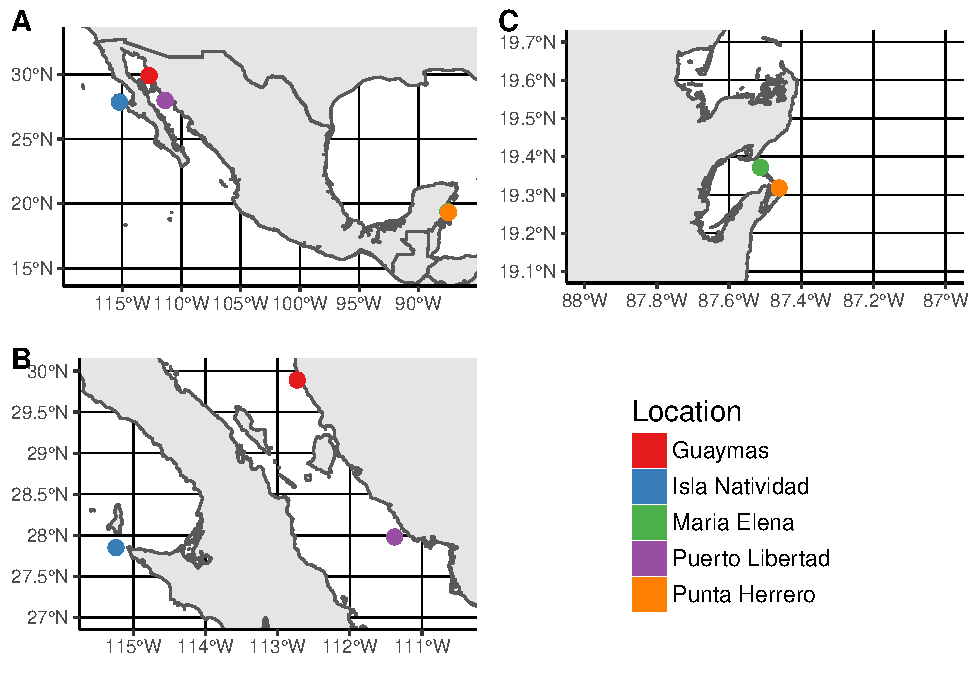
\includegraphics{Villasenor-Derbez_files/figure-latex/create_map-1.pdf}
\caption{(\#fig:create\_map)\label{fig:map}Mapa de la localización
general de las comunidades de estudio. El panel de la derecha es un
acercamiento a las comunidades de María Elena y Punta Herrero.}
\end{figure}

\subsection{Data collection}\label{data-collection}

\subsection{Data analysis}\label{data-analysis}

\subsubsection{Biological}\label{biological}

Table \ref{table:indicators} is the way to cite a table.

\begin{table}

\caption{\label{tab:unnamed-chunk-2}\label{table:indicators}Lista de indicadores utilizados para evaluar resvas marinas, agrupados por tipo.}
\centering
\begin{tabular}[t]{l|l}
\hline
Category & Indicador\\
\hline
Biological & Índice de diversidad de shannon\\
\hline
Biological & Riqueza\\
\hline
Biological & Densidad\\
\hline
Biological & Nivel trófico\\
\hline
Biological & Biomasa\\
\hline
Biological & Densidad de especies objetivo\\
\hline
Socioeconomic & Ingresos por especies objetivo\\
\hline
Socioeconomic & Arribos de especies objetivo\\
\hline
Governance & Tipo de acceso a la pesquería\\
\hline
Governance & Grado de pesca ilegal\\
\hline
Governance & Procuración de la reserva\\
\hline
Governance & Tipo de organización pesquera\\
\hline
Governance & Edad de la reserva\\
\hline
\end{tabular}
\end{table}

\subsubsection{Socioeconomic}\label{socioeconomic}

\subsubsection{Governance}\label{governance}

\section{Results}\label{results}

\includegraphics{Villasenor-Derbez_files/figure-latex/unnamed-chunk-3-1.pdf}

\section{Discussion}\label{discussion}

This section may be divided by subheadings. Discussions should cover the
key findings of the study: discuss any prior art related to the subject
so to place the novelty of the discovery in the appropriate context;
discuss the potential short-comings and limitations on their
interpretations; discuss their integration into the current
understanding of the problem and how this advances the current views;
speculate on the future direction of the research and freely postulate
theories that could be tested in the future.

Summary of main findings Limitations Conclusions

\section*{Conflict of Interest Statement}

The authors declare that the research was conducted in the absence of
any commercial or financial relationships that could be construed as a
potential conflict of interest.

\section*{Author Contributions}

JC analyzed and interpreted data, discussed the results and wrote the
manuscrip. SF and JT edited the manuscript and discussed the results.

\section*{Funding}

Details of all funding sources should be provided, including grant
numbers if applicable. Please ensure to add all necessary funding
information, as after publication this is no longer possible.

\section*{Acknowledgments}

This is a short text to acknowledge the contributions of specific
colleagues, institutions, or agencies that aided the efforts of the
authors.

\section*{Supplemental Data}

\href{http://home.frontiersin.org/about/author-guidelines#SupplementaryMaterial}{Supplementary Material}
should be uploaded separately on submission, if there are Supplementary
Figures, please include the caption in the same file as the figure.
LaTeX Supplementary Material templates can be found in the Frontiers
LaTeX folder

\paragraph*{S1 Figure}
\label{S1_Figure}

Maps of the marine reserves and corresponding control sites at each
community.

\paragraph*{S2 Table}
\label{S2_Table}

Table with a general overview of on the governance characteristics of
each community.

\bibliographystyle{frontiersinSCNS_ENG_HUMS}\bibliography{references}

\section*{Figure captions}



\end{document}
